\subsection{Cyclotron mass}
To extract the cyclotron mass from the Chambers model, we need a new approach. In contrast to the
Drude model, here we do not have the cyclotron frequency as an explicit parameter of the formula.
We cannot use the effective mass from the dispersion relation of the tight-binding model either;
It is equal to
\begin{equation}
    m^* = \hbar^2\qty(\pdv[2]{\varepsilon}{k})^{-1}
\end{equation}
and varies for different parts of the dispersion relation. In order to define a useful parameter,
we need to average over the wavevectors. So
\begin{equation}
    m_c = \frac{\hbar}{2\pi}\oint\frac{\dd{k}}{v_\perp (k)}
\end{equation}
where $v_\perp$ is the velocity perpendicular to the magnetic field, on the path the charge
carriers take.\footnote{This is a closed path on the Fermi surface, since the magnetic field does
not do work and the free charges are on the Fermi surface. The path is closed due to the periodic
nature of the oscillations.}

\begin{figure}
    \centering
    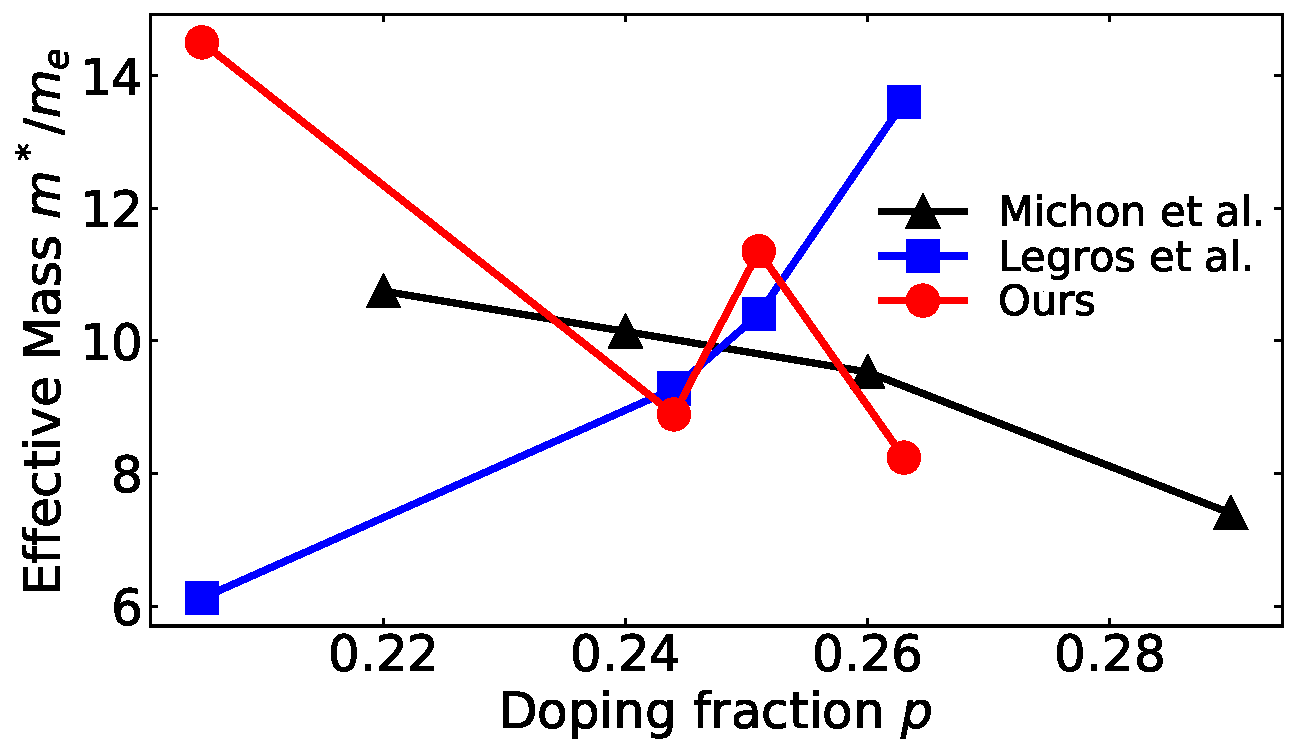
\includegraphics[width=0.7\textwidth]{figures/effective_mass}
    \caption{Comparison of our calculated effective masses with Michon et al. and Legros et al.}
    \label{fig:effective_mass}
\end{figure}

In Figure \ref{fig:effective_mass}, we present our final results for the effective mass and compare
them with the results of Michon et al. and Legros et al. Due to data unavailability, we have very
few points for comparison, so drawing strong conclusions is difficult. However, we can see that
our results are qualitatively closer to Michon et al., in the sense that the effective mass does
not decrease and increase as much in low and high doping respectively, and that it is roughly
decreasing in the measured range like Michon et al. Again, the data is very sparse and there are
large errors, so these conclusions are not definitive.
